\documentclass[a4paper,
fontsize=11pt,
%headings=small,
oneside,
numbers=noperiodatend,
parskip=half-,
bibliography=totoc,
final
]{scrartcl}

\usepackage{synttree}
\usepackage{graphicx}
\setkeys{Gin}{width=.4\textwidth} %default pics size

\graphicspath{{./plots/}}
\usepackage[ngerman]{babel}
\usepackage[T1]{fontenc}
%\usepackage{amsmath}
\usepackage[utf8x]{inputenc}
\usepackage [hyphens]{url}
\usepackage{booktabs} 
\usepackage[left=2.4cm,right=2.4cm,top=2.3cm,bottom=2cm,includeheadfoot]{geometry}
\usepackage{eurosym}
\usepackage{multirow}
\usepackage[ngerman]{varioref}
\setcapindent{1em}
\renewcommand{\labelitemi}{--}
\usepackage{paralist}
\usepackage{pdfpages}
\usepackage{lscape}
\usepackage{float}
\usepackage{acronym}
\usepackage{eurosym}
\usepackage[babel]{csquotes}
\usepackage{longtable,lscape}
\usepackage{mathpazo}
\usepackage[normalem]{ulem} %emphasize weiterhin kursiv
\usepackage[flushmargin,ragged]{footmisc} % left align footnote
\usepackage{ccicons} 

%%%% fancy LIBREAS URL color 
\usepackage{xcolor}
\definecolor{libreas}{RGB}{112,0,0}

\usepackage{listings}

\urlstyle{same}  % don't use monospace font for urls

\usepackage[fleqn]{amsmath}

%adjust fontsize for part

\usepackage{sectsty}
\partfont{\large}

%Das BibTeX-Zeichen mit \BibTeX setzen:
\def\symbol#1{\char #1\relax}
\def\bsl{{\tt\symbol{'134}}}
\def\BibTeX{{\rm B\kern-.05em{\sc i\kern-.025em b}\kern-.08em
    T\kern-.1667em\lower.7ex\hbox{E}\kern-.125emX}}

\usepackage{fancyhdr}
\fancyhf{}
\pagestyle{fancyplain}
\fancyhead[R]{\thepage}

% make sure bookmarks are created eventough sections are not numbered!
% uncommend if sections are numbered (bookmarks created by default)
\makeatletter
\renewcommand\@seccntformat[1]{}
\makeatother


\usepackage{hyperxmp}
\usepackage[colorlinks, linkcolor=black,citecolor=black, urlcolor=libreas,
breaklinks= true,bookmarks=true,bookmarksopen=true]{hyperref}
%\usepackage{breakurl}

%meta
%meta

\fancyhead[L]{V. Hillebrand\\ %author
LIBREAS. Library Ideas, 34 (2018). % journal, issue, volume.
\href{http://nbn-resolving.de/}
{}} % urn 
% recommended use
%\href{http://nbn-resolving.de/}{\color{black}{urn:nbn:de...}}
\fancyhead[R]{\thepage} %page number
\fancyfoot[L] {\ccLogo \ccAttribution\ \href{https://creativecommons.org/licenses/by/4.0/}{\color{black}Creative Commons BY 4.0}}  %licence
\fancyfoot[R] {ISSN: 1860-7950}

\title{\LARGE{„Weil ich glaube, die wenigsten wollen überhaupt in die Forschung gehen … “}}% title
\subtitle{Entwicklung der aktuellen Studienordnungen am IBI}
\author{Vera Hillebrand} % author

\setcounter{page}{1}

\hypersetup{%
      pdftitle={„Weil ich glaube, die wenigsten wollen überhaupt in die Forschung gehen … “ : Entwicklung der aktuellen Studienordnungen am IBI},
      pdfauthor={Vera Hillebrand},
      pdfcopyright={CC BY 4.0 International},
      pdfsubject={LIBREAS. Library Ideas, 34 (2018).},
      pdfkeywords={Bibliothekswissenschaft, Institut für Bibliotheks- und Informationswissenschaft, Humboldt-Universität zu Berlin, Studienordnung, Bachelor, Master, Umfrage},
      pdflicenseurl={https://creativecommons.org/licenses/by/4.0/},
      pdfcontacturl={http://libreas.eu},
      baseurl={http://libreas.eu},
      pdflang={de},
      pdfmetalang={de}
     }

\date{}
\begin{document}

\maketitle
\thispagestyle{fancyplain} 

%abstracts
\begin{abstract}
In den letzten zwei Jahren veröffentlichte das Institut für Bibliotheks-
und Informationswissenschaft (IBI) zwei neue Studienordnungen, einmal
für den Bachelorstudiengang Bibliotheks- und Informationswissenschaft,
einmal für den Master Information Science. Dieser Artikel referiert die
Argumente und Überlegungen am Institut zur Konzeption neuer
Studienordnungen und beschreibt die begleitende Umfrage unter und
Fokusgruppen mit Studierenden.
\end{abstract}

%body
In den letzten zwei Jahren veröffentlichte das Institut für Bibliotheks-
und Informationswissenschaft (IBI) zwei neue Studienordnungen, einmal
für den Bachelorstudiengang Bibliotheks- und Informationswissenschaft,
einmal für den Master Information Science. Dieser Artikel referiert die
Argumente und Überlegungen am Institut zur Konzeption neuer
Studienordnungen und beschreibt die begleitende Umfrage unter und
Fokusgruppen mit Studierenden.

In der aktuellen Ausgabe von Bibliothek, Wissenschaft und Praxis
hinterfragt Ragnar Andreas Audunson (Audunson, 2018, S. 359) die
Ausbildung in der Bibliotheks- und Informationswissenschaft:
\emph{\enquote{Which part of the knowledge base and curriculum of our
program are robust and relevant, which are of a more ephemeral nature?}}
Dieser Wunsch nach robusten Inhalten bezieht sich auf seine eigene
Ausbildung in den 1980ern, in der er Kurse in \emph{library automation}
hatte. Ein Themenfeld, das er persönlich inzwischen für völlig überholt
hält, während das Fach \emph{indexing theory} ihm noch heute relevante
Kompetenzen vermittelte. Während der Vorbereitung für das 90-jährige
Jubiläum des Instituts für Bibliotheks- und Informationswissenschaft
(IBI) stieß man im Archiv der Humboldt-Universität zu Berlin auf den
Stundenplan des ersten Wintersemesters 1928/29 im Fachbereich
Bibliothekswissenschaft am heutigen IBI. Auch hier kann darüber
geurteilt werden, was robuste und relevante Inhalte und welche Inhalte
vergänglicher Natur sind, auch wenn dieses Urteil mit hoher
Wahrscheinlichkeit nicht immer gleich ausfällt. Bis auf Urheberrecht
finden sich keine der damaligen Themen in den aktuellen Studienordnungen
wieder. Alle Studienordnungen seit 2005 für den Bachelor- und
Masterstudiengang im Direktstudium am Institut für Bibliotheks- und
Informationswissenschaft sind neben den Ordnungen anderer Studiengänge
auf der Webseite der Humboldt-Universität einsehbar.\footnote{\url{https://gremien.hu-berlin.de/de/amb?selectedType=Studienordnung\#B}}

\begin{figure}
\centering
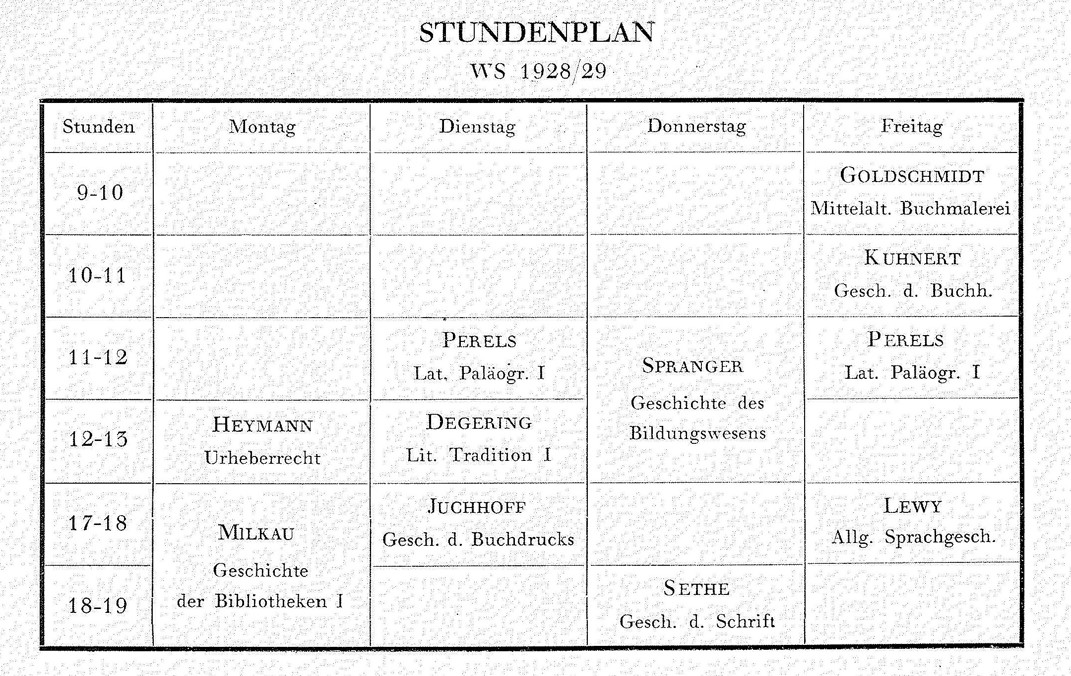
\includegraphics[width=10cm]{img/Abb1.jpg}
\caption{Stundenplan des Institutes für Bibliothekswissenschaft für das
WS 1928/29}
\end{figure}

Ein Grund für die neuen Studienordnungen im Bachelor und Master bestand
insbesondere darin, dass in den letzten sieben Jahren ein reger Wechsel
bei den ProfessorInnen- und DozentInnenstellen des Instituts
stattgefunden hat. Von 2011 bis 2018 verabschiedete das IBI Prof.~
Dr.~Konrad Umlauf, Prof.~Dr.~Peter Schirmbacher, Dipl. Math. Michael
Heinz, Dr.~Gertrud Pannier und zuletzt Prof.~Michael Seadle, PhD, in den
Ruhestand. Ferner verließ Prof.~Dr.~Gradmann nach einem externen Ruf das
IBI. All diese Persönlichkeiten hinterließen in der Modulplanung
Einschnitte, vor allem da mit ihnen auch vier Lehrstühle das IBI
verließen: Öffentliche Bibliotheken (Prof.~Umlauf),
Informationsmanagement (Prof.~Schirmbacher), Wissensmanagement (
Prof. Gradmann) und Digitale Bibliotheken (Prof.~Seadle). In den letzten
sieben Jahren gab es aber nicht nur Verabschiedungen, sondern auch drei
Neuzugänge bei den Professuren: Prof.~Vivien Petras, PhD, die 2014 die
Tenure auf ihre Juniorprofessorenstelle bekommen hatte, Prof.~Dr. Elke
Greifeneder, die 2014 den Lehrstuhl Information Behavior gründete und
Prof.~Dr.~Robert Jäschke, der seit 2017 den Lehrstuhl Information
Processing and Analytics aufbaut. Für die Zukunft sind weitere
Professuren im Bereich Information Management und Data \& Information
Literacy geplant. Damit wird es insgesamt fünf Professuren geben, die
den Lehrplan der Studiengänge ausgestalten.

Diese Entwicklung bedeutete eine Veränderung des Studienverlaufes, da
die ProfessorInnen mit ihren Forschungsthemen die Lehre nachhaltig
prägen. Es war den Lehrenden wichtig zu wissen, wie die Sicht der
Studierenden auf die zukünftige Entwicklung des Studiums ist. Die
Entwicklung der neuesten Studienordnungen des Bachelorstudienganges 2017
und des Masterstudienganges 2018 wurden daher von dem Projektseminar
\enquote{Evaluierung der Studienordnungen am IBI} begleitet. 14
Bachelor- und Masterstudierende entwarfen im Rahmen des Seminars einen
Fragebogen und führten zwei Fokusgruppen durch, um folgende Fragen zu
beantworten: Wie bewerten Studierende das Studium am IBI? Welche Kritik
und Wünsche gibt es, die in die Planung der zukünftigen Studiengänge mit
aufgenommen werden können? Betreut von Prof.~Elke Greifeneder und ihrer
wissenschaftlichen Mitarbeiterin Kirsten Schlebbe erhielten die
Studierenden eine Einführung in die Durchführung von quantitativen
Umfragen und qualitativen Fokusgruppen.

\hypertarget{konzeption-der-umfrage-unter-studierenden}{%
\section{Konzeption der Umfrage unter
Studierenden}\label{konzeption-der-umfrage-unter-studierenden}}

Bei der Konzipierung des Fragebogens stellte die größte Herausforderung
dar, wie man am besten die Studierenden unterschiedlicher Fachsemester
nach der Bewertung der bereits existierenden Module befragen könnte, da
Studierende im Master sich möglicherweise nicht mehr genau daran
erinnern konnten, worum es in einem Modul ging beziehungsweise durch den
langen Abstand eine andere Haltung zu Inhalten eingenommen haben könnten
und Studierende im ersten oder zweiten Semester im Bachelor gerade erst
Module besucht hatten, also die Erinnerungen sehr frisch waren, aber
eben ohne die zeitliche \enquote{Reife} und manche Module schlichtweg
noch nicht besucht wurden. Diese Befragung sollte daher explizit nicht
wie eine Evaluation am Ende des Semesters gestaltet sein. Der Fokus lag
auf den Inhalten, die in den Modulen laut Studienordnung vermittelt
werden sollten.

Nach der Betrachtung und Zusammenfassung der Themenbereiche der
Studienordnungen, ausgiebigen Diskussionen im Seminar und der
Kontaktaufnahme mit den Lehrenden des IBI wurden schließlich 45
Themenfelder festgelegt, welche die zu vermittelnden Inhalte der
Studienordnung widerspiegeln. Die Studierenden entschieden sich für eine
zweistufige Evaluation. Im ersten Schritt sollten die Teilnehmenden
angeben, mit welchen Themengebieten sie während ihres Studiums am IBI
bereits in Berührung gekommen sind. Im zweiten Schritt sollten sie
entscheiden, welche von den ihnen bereits bekannten Themen sie als
wichtig erachten. Zusätzlich wurde ein Freitextfeld eingerichtet, durch
das Studierende die Möglichkeit hatten, Themen zu nennen, welche ihnen
bisher im Studium fehlten. An diesem Punkt diskutierten die Studierenden
über die Schwächen der quantitativen Methode und deren Auswirkungen auf
die Ergebnisse: Welche Aspekte werden von individuellen Studierenden als
wichtiger erachtet und in welchem Zusammenhang? Was, wenn Studierende
Themenbereiche angeben, mit denen sie laut Studienverlaufsplan gar nicht
in Berührung hätten kommen können? Welche Rolle spielt die eigene
außeruniversitäre Bildung in der Entscheidung nach Wichtigkeit? Um die
Ergebnisse besser einordnen zu können, wurden die Teilnehmenden gebeten,
Angaben zu außeruniversitären beziehungsweise vorherigen Ausbildungen,
zum Studienverlauf und zu ihrer Studien- und Prüfungsordnung zu machen.

Um festzustellen, ob die Entscheidung der Wichtigkeit von der eigenen
beruflichen Zukunftsperspektive beeinflusst wird, entschieden sich die
Studierenden die Frage zu stellen, in welchem Bereich man später
arbeiten möchte. Als Antwortmöglichkeiten standen
Bibliothekswissenschaft, Informationswissenschaft oder ein Freitextfeld
zur Auswahl. Damit waren nicht alle Studierenden gänzlich glücklich und
es wurde zusätzlich eine freie Frage nach dem zukünftigen Arbeitsplatz
gestellt: Wenn Sie frei wählen könnten, wo würden Sie nach Ihrem
Studienabschluss gerne arbeiten?

Ein eigenständiger Block im Fragebogen konzentrierte sich auf die Frage
nach der Rolle der Praxis in der Lehre am IBI. Mit Praxis waren
Veranstaltungsformen wie Exkursionen, Tutorien, Praktikum und
Projektseminare gemeint. Solche Veranstaltungen sollen Studierenden die
Möglichkeit geben, Erfahrungen zu machen oder Kenntnisse zu gewinnen
beziehungsweise zu verbessern, die theoretische Inhalte von Vorlesungen
und Seminaren nicht abdecken. Es wurde in diesem Zusammenhang nach der
Beurteilung des Umfangs der einzelnen Veranstaltungsformen am IBI
gefragt.

Der Fragebogen schloss mit demographischen Angaben zu Geschlecht und
Alter. Die Befragung war insgesamt drei Wochen aktiv, sowohl online als
auch in gedruckter Form. 121 Studierende nahmen an der Umfrage teil, das
sind circa 30\,\% der Studierenden aus den Direktstudiengängen am IBI.

\hypertarget{konzeption-und-teilnehmer-der-fokusgruppen}{%
\section{Konzeption und Teilnehmer der
Fokusgruppen}\label{konzeption-und-teilnehmer-der-fokusgruppen}}

Die Teilnehmenden des Fragebogens konnten am Ende der Umfrage ihre
E-Mailadresse hinterlegen, wenn sie Interesse an der Mitarbeit in einer
Fokusgruppe hatten. Bachelor- und Masterstudierende sollten getrennt mit
jeweils 6--7 Personen an einer Fokusgruppe teilnehmen (Details zu den
TeilnehmerInnen siehe Tabelle 1). Ziel der Fokusgruppen war es,
Ergebnisse des Fragebogens aufzugreifen und weiterführende Erklärungen
für Ergebnisse zu bekommen. Nach der Warm-up Phase, in der die
Teilnehmenden darüber sprachen, wieso sie sich für das Studium am IBI
entschlossen hatten, widmete sich der erste Block des Gesprächs der
Frage nach dem Praxisanteil im Studium. Die bereits existierenden
Tutorien wurden besprochen und erfragt, wie diese von den Studierenden
aufgenommen werden. Danach wurden mit den TeilnehmerInnen die Ergebnisse
des Fragebogens diskutiert. Der Fokus lag dabei auf den Themenbereichen,
die mehr als 30\,\% der Bachelorstudierenden und mehr als 25\,\% der
Masterstudierenden im Rahmen der Umfrage als \emph{\enquote{nicht
wichtig}} beurteilt hatten. Zuletzt sprachen die Moderierenden das
Verhältnis zwischen Informations- und Bibliothekswissenschaft an. Diesem
Teil der Fokusgruppen ging voraus, dass es bereits intern bei der
Erstellung des Fragebogens zur Diskussion kam, wie viele der
Studierenden am IBI sich am Ende ihres Studiums in einer Bibliothek oder
einer Einrichtung sehen, zu der ein bibliothekswissenschaftlicher
Hintergrund passt, und wie viele sich eher der
informationswissenschaftlichen, technischen Seite zugeneigt finden. Die
ProfessorInnen wollten wissen, wie Studierende zu der Idee stehen, dass
diese Zweige in den Modulen voneinander gelöst werden, um die
Interessierten besser auf ihre berufliche Perspektive vorzubereiten. Zum
Schluss wurden die Studierenden nach ihren Wünschen in Bezug auf das
Studium am IBI gefragt.

\pagebreak

\begin{longtable}[]{@{}llccc@{}}
\toprule
& Geschlecht & Fachsemester & FaMI-Ausbildung & BA am IBI\tabularnewline
\midrule
\endhead
Fokusgruppe Bachelor & & & &\tabularnewline
\midrule
Teilnehmer 1 & weiblich & 4 & &\tabularnewline
Teilnehmer 2 & weiblich & 6 & &\tabularnewline
Teilnehmer 3 & weiblich & 6 & &\tabularnewline
Teilnehmer 4 & männlich & 4 & x &\tabularnewline
Teilnehmer 5 & weiblich & 2 & x &\tabularnewline
Teilnehmer 6 & weiblich & 4 & &\tabularnewline
\midrule
Fokusgruppe Master & & & &\tabularnewline
\midrule
Teilnehmer 1 & weiblich & 2 & x & x\tabularnewline
Teilnehmer 2 & männlich & 4 & & x\tabularnewline
Teilnehmer 3 & weiblich & 2 & x &\tabularnewline
Teilnehmer 4 & weiblich & 2 & & x\tabularnewline
Teilnehmer 5 & weiblich & 2 & & x\tabularnewline
Teilnehmer 6 & männlich & 4 & &\tabularnewline
Teilnehmer 7 & weiblich & 4 & & x\tabularnewline
\bottomrule
\caption{Übersicht der Teilnehmenden der Fokusgruppen}
\end{longtable}


\hypertarget{ergebnisse}{%
\section{Ergebnisse}\label{ergebnisse}}

111 der 121 TeilnehmerInnen studierten Bibliotheks- und
Informationswissenschaft, davon der größte Teil im Bachelor
(72).\footnote{Die übrigen 10 Studierenden gehören dem Studiengang
  Informationsmanagement und Informationstechnologie an, dessen
  Studienverlauf sich mit unserem überschneidet.} Auch studierte die
Mehrheit in der damalig aktuellsten Studienordnung von 2014 (80). 40
Studierende kamen direkt vom Abitur ans IBI, 33 waren vorher beruflich
tätig und 28 hatten zuvor bereits ein Studium absolviert oder
abgebrochen. Der Hauptteil der Befragten war zur Zeit der Umfrage 21--30
Jahre alt (78) und 80 von ihnen waren weiblich. Mit 121 Fragebögen deckt
die Umfrage circa 1/3 der gesamten Studierenden am IBI ab und spiegelt
auch die gefühlte Realität wieder: mehrheitlich weibliche Studierende,
mit heterogenem Hintergrund und einer großen Altersspanne.

Auf die Frage nach der beruflichen Perspektive ergaben sich drei
Ausprägungen: 1) Zu bibliothekswissenschaftlichen (50 Studierende, 42\,\%)
und 2) informationswissenschaftlichen Einrichtungen (44 Studierende,
36\,\%) fühlen sich jeweils ungefähr gleich viele Studierenden hingezogen.
26 (22\,\%) Teilnehmende gaben im Freitextfeld eine ganz andere
Berufsperspektive an.

Mit dem Praxisangebot bei Projektseminaren, Exkursionen und Praktikum
waren jeweils circa 50\,\% der Studierenden zufrieden. Bei den Tutorien
gaben 43\,\% an, es könnte mehr davon geben.

Bei der Auswertung der Themenfächer stellte die Seminargruppe fest, dass
einige Probleme der angewandten Methodik nicht zur Gänze hatten gelöst
werden können: Die Verbindung zwischen Lehrenden und Inhalt sollte für
die Erhebung der Studieninhalte aufgelöst werden. Es wurde mehrfach
schriftlich wie mündlich betont, dass es bei der Umfrage nicht um die
Lehrenden, sondern um die Bewertung der Lehrinhalte ginge. Aber
spätestens bei den Fokusgruppen stellen die Seminargruppe fest, dass das
nicht funktionierte. In vielen Fällen merkte man die deutliche Färbung
durch den Dozierenden, die die Studierenden zum Urteil \enquote{wichtig}
oder \enquote{unwichtig} brachten.

Auch musste immer wieder zum Ausgangspunkt zurückgekehrt werden, dass es
keine ausschlaggebende Meinung ist, wenn ein Themenschwerpunkt mit hohen
Prozentzahlen als unwichtig eingestuft wurde, jedoch nur eine Minderheit
der Gesamtmenge damit zu tun hatte. Ein Beispiel aus dem Bachelor: 48\,\%
fanden das Thema Forschungsorganisation unwichtig, aber nur 23
Studierende hatten dazu Kurse besucht, dagegen hatten 48 Kurse zu Aufbau
und Arbeitsweisen von Rechnern gehabt und 40\,\% davon fanden dies
unwichtig. Es wäre nicht gerechtfertigt daraus zu schlussfolgern, dass
das eine oder andere Thema wichtiger für den Studiengang sei. Für diesen
Artikel werden daher nur jene Themenbereiche analysiert, bei denen
mindestens 90\,\% der Befragten angaben, Kurse dazu besucht zu haben.

Bei den Bachelorstudierenden sind es Programmiersprachen und
Formalerschließung, die am häufigsten als unwichtig eingestuft wurden:
Programmiersprachen von 19 der 67 Personen und Formalerschließung von 15
der 69 Personen, die Angaben mit dem Thema während ihres bisherigen
Studiums in Kontakt gekommen zu sein (Tabelle 2).

%\pagebreak


\begin{longtable}[]{@{}p{3.5cm}p{9cm}p{2.5cm}@{}}
\toprule
\multicolumn{3}{l}{\textbf{Bachelor/n=72, Angaben mit mindestens 90\,\% Beteiligung}}\\
\midrule
\endfirsthead
\endhead
Angabe \enquote{in Berührung gekommen} \newline in Personen & Themenschwerpunkt &
Angabe \newline \enquote{unwichtig}\\
\midrule
\centering 67 & Programmiersprachen & \centering 28\,\% \tabularnewline
\centering 69 & Formalerschließung & \centering 22\,\% \tabularnewline
\centering 68 & Inhaltserschließung/ Informationsaufbereitung &  \centering15\,\%\tabularnewline
\centering 68 & Information Retrieval &  \centering15\,\% \tabularnewline
\centering 65 & Usability & \centering 15\,\% \tabularnewline
\centering 65 & Open Access & \centering 11\,\% \tabularnewline
\centering 68 & Datenformate & \centering 11\,\% \tabularnewline
\centering 66 & Metadaten & \centering 9\,\% \tabularnewline
\bottomrule
\caption{Bewertungen der Themenfelder im Bachelor, mit denen mehr als 90\,\% der Befragten in Kontakt kamen}
\end{longtable}

Bei den Masterstudierenden gibt es generell weniger starke Aussagen.
Metadaten, Informationssysteme, Dienstleistungen und Inhaltliche
Erschließung wurden von jeweils 7\,\% der Befragten als
\enquote{unwichtig} eingestuft. Das sind umgerechnet 4 von 30 Personen,
die diese Auswahl trafen (Tabelle 3).

\pagebreak

\begin{longtable}[]{@{}p{3.5cm}p{9cm}p{2.5cm}@{}}
\toprule
\multicolumn{3}{l}{\textbf{Master/n=30, Angaben mit mindestens 90\,\% Beteiligung}} \\
\midrule
\endhead
Angabe \enquote{in Berührung gekommen} \newline in Personen & Themenschwerpunkt &
Angabe \newline \enquote{unwichtig}\tabularnewline
\midrule
\centering 29 & Metadaten & \centering 7\,\%\tabularnewline
\centering 28 & Informationssysteme und Dienstleistungen & \centering 7\,\%\tabularnewline
\centering 28 & Inhaltliche Erschließung/ Informationsaufbereitung & \centering 7\,\%\tabularnewline
\centering 27 & Statistik & \centering 4\,\%\tabularnewline
\centering 27 & Open Access & \centering 4\,\%\tabularnewline
\centering 28 & Suchstrategien und Suchquellen & \centering 4\,\%\tabularnewline
\centering 29 & Information Retrieval & \centering 0\,\%\tabularnewline
\bottomrule
\caption{Bewertungen der Themenfelder im Master, mit denen mehr als
90\,\% der Befragten in Kontakt kamen}
\end{longtable}

Die Ergebnisse der Fokusgruppen bestätigten, dass sich Studierende mehr
studienbegleitende Tutorien wünschen. Oft wurde dies damit begründet,
dass neben der Theorie zu wenig Zeit für das Ausprobieren und Erlernen
der praktischen Umsetzung bliebe. Beim Thema Praktikum setzte sich in
der Bachelorgruppe die Meinung der anwesenden ehemaligen
Fachangestellten für Medien- und Informationsdienste (FaMis) durch, die
das Praktikum für zu kurz hielten. Einige Teilnehmenden der Mastergruppe
waren ebenfalls dieser Meinung. Beide Gruppen scheiterten aber an einem
einstimmigen Ergebnis, da klar war, dass ein längeres Praktikum im
Studium nur schwer umsetzbar sei, vor allem, da es zu viele unbezahlte
Praktika gäbe. Ein klarer Widerspruch kam aus der Bachelorgruppe, als
das Thema Formalerschließung als \enquote{unwichtiger} Themenschwerpunkt
besprochen wurde. Auch hier vor allem von der \enquote{FaMi-Seite}.
Generell lässt sich sagen, dass in keiner der beiden Fokusgruppen ein
Thema von einer Mehrheit als völlig unwichtig bewertet wurde. Viel öfter
ging es um die Frage, ob etwas ein Pflichtthema sein sollte oder eher
etwas für den Wahlpflichtbereich sei. Überraschend für die
Projektseminargruppe waren die Aussagen der Bachelorstudierenden, dass
das Thema \enquote{Wissenschaftliches Fehlverhalten} zwar wichtig sei,
aber viel zu oft behandelt worden wäre. Bei den Masterstudierenden waren
sich die Studierenden einig, dass Medien- und Buchgeschichte zwar
\enquote{ganz nett} sei, aber nicht zwingend notwendig für den
Studiengang. Alle Themen, die mit Forschung zu tun hatten, wurden dem
Masterstudiengang zugeschrieben.

\begin{quote}
\textbf{\enquote{{[}\ldots{}{]} so etwas hätte ich eigentlich eher in
den Master gepackt. Also, in dem Moment, in dem man mir sagt, ich hänge
einen Master dran, dann sagt man schon, dass man wissenschaftlicher
arbeiten will.} (BA-Gruppe, T4)}
\end{quote}

Ein Gesprächsblock entstand aus den Freitextfeldangaben zu den Themen,
die den Studierenden am IBI noch fehlten: Programmieren,
Bibliotheksmanagement und Datenbanken. Diese Themen waren zwar bereits
in die Studienordnung 2014 integriert, aber da sie häufig genannt worden
waren, wollten wir von den Fokusgruppen wissen, wie sie besser in die
neue Studienordnung eingearbeitet werden könnten. Die
Bachelorstudierenden sahen Datenbanken und Programmieren im
Wahlpflichtbereich und fanden Bibliotheksmanagement durch das bereits
existierende Wahlpflichtmodul abgedeckt. Stattdessen wünschte man sich,
mehr über den Ablauf in Bibliotheken zu lernen. Ein gegenteiliges Bild
zeichnete sich im Master ab, dort forderte man mehr Programmieren mit
einem anwendungsbezogenen Ansatz. Dasselbe für Datenbanken, gewünscht
wurde ein Pflichtmodul. Bibliotheksmanagement, ein Themenbereich, der in
der Master-Studienordnung von 2014 nicht gelehrt wird, wurde von einem
Masterstudierenden kommentiert:

\begin{quote}
\textbf{\enquote{{[}\ldots{}{]} wenn hier die Absolventen befähigt sein
sollten, irgendwann die Leitung von Bibliotheken zu übernehmen, dann
finde ich es erschreckend, dass sowohl im Bachelor, als auch im Master
kein Management-Modul Pflicht ist.} (MA-Gruppe, T6)}
\end{quote}

Die Emotionen kochten in beiden Gruppen bei der Frage hoch, ob es besser
wäre, die bibliothekswissenschaftlichen von den
informationswissenschaftlichen Inhalten im Studium zu trennen. Es gab
überwiegend eine Ablehnung dieser Idee in beiden Gruppen:

\begin{quote}
\textbf{\enquote{{[}\ldots{}{]} wir sind eine neue Generation von
Bibliothekaren, {[}\ldots{}{]} unser Berufsfeld hat sich einfach
deutlich vergrößert, einfach weil wir eben mit Daten arbeiten und
theoretisch kannst du halt überall landen heutzutage mit dem Studium
{[}\ldots{}{]}, aber ich glaube es bringt einem beruflich am Ende mehr,
diese ganzen Sachen mal gemacht zu habe {[}\ldots{}{]}} (BA-Gruppe, T4)}

\textbf{\enquote{{[}\ldots{}{]} finde ich es ja auch gut, dass wir diese
ganzen Sachen haben und dass der Studiengang beides auch verpflichtend
macht. Aber sonst bleibt man ja immer so ein bisschen in seiner
Komfortzone drin. Wenn ich jetzt zum Beispiel weiß, ich möchte eher in
so eine Informatiker-Richtung gehen, dann mache ich natürlich nur die
Kurse, die irgendwie mehr Informatik sind {[}\ldots{}{]}} (MA-Gruppe,
T2)}
\end{quote}

Jedoch gab es auch vereinzelte Stimmen, die Argumente für eine Trennung
sahen:

\begin{quote}
\textbf{\enquote{Deswegen, eigentlich gerade aus den Argumenten, die du
gerade gesagt hast, bin ich eigentlich für die Trennung, muss ich sagen,
also einfach weil wir gerade eine neue Generation sind und ich einfach
das gerade schön finde. Na wenn ich wirklich Daten sortiere, dann sehe
ich mich nicht mehr als Bibliothekar, muss ich ganz ehrlich sagen.}
(BA-Gruppe, T6)}

\textbf{\enquote{Also es ist einfach nicht eine Einheit, sondern die
Trennung ist ganz klar da. Und das sieht man auch an den
Studierendenprofilen, die es so gibt.} (MA-Gruppe, T5)}
\end{quote}

In der Bachelorgruppe eröffnete sich eine Lösung in weniger Pflicht- und
mehr Wahlpflichtmodulen, um den Studierenden selbst die Wahl zu lassen,
in welche Richtung sie sich entwickeln wollen. Dies befürwortenden vor
allem jene, die noch nicht genau wussten, welchen Beruf sich nach dem
Studium ergreifen möchten.

\begin{quote}
\textbf{\enquote{Sozusagen, ich finde, ganz zu Anfang sollte man beides
mal bis zu einem gewissen Grad gemacht haben, einfach weil ich wusste
zum Beispiel nicht, was ich wollte, mit diesem Studium.} (BA-Gruppe,
T6)}
\end{quote}

Ein Thema, das ähnlich diskutiert wurde, war der allgemeine Praxisanteil
des universitären Studiums. Es wurde sich über den zu hohen
Theorieanteil im Studium beklagt, mit dem Verständnis, dass Theorie vor
allem für die Forschung wichtig sei und nicht jeder Studierende später
in der Forschung arbeiten möchte. Mit Praxis waren neben mehr Tutorien
oder Übungen auch mehr Projekte, sei es in Seminaren oder außerhalb,
erwünscht.

Weitere Ergebnisse aus den beiden Studien wurden in einem
BBK-Vortrag\footnote{Saß, Nico und Hillebrand, Vera (2016) : Evaluierung
  der Lehrinhalte am IBI. Abrufbar auf der BBK Webseite: \href{http://www.ibi.hu-berlin.de/de/bbk/abstracts/ws1617/eva}{http://www.ibi.hu-berlin.de/de/bbk/abstracts/ws1617/eva}.}
im Herbst 2016 vorgetragen.

%\pagebreak

\section{Die neuen Studienordnungen des IBI}

Ungefähr ein Jahr nach dem Projektseminar trat die Studienordnung 2017
für den Bachelor in Kraft, die sich aus fünf Pflichtmodulen und fünf
Wahlpflichtmodulen zusammensetzt (Tabelle~4).

\begin{longtable}[]{@{}p{8cm}p{8cm}@{}}
\toprule
\multicolumn{2}{l}{\textbf{Studienordnung Bachelor Bibliotheks- und Informationswissenschaft 2017}} \tabularnewline
\midrule
\endhead
Pflichtmodule & Wahlpflichtmodule\tabularnewline
\midrule
BP1: Einführung in die Bibliotheks- und Informationswissenschaft & BWP1:
Informationsdidaktik\tabularnewline
BP2: Informations- und Kommunikationstechnologie & BWP2: Information
Processing and Storage\tabularnewline
BP3: Informationsproduktion und \-manage\-ment & BWP3: Information und
Gesellschaft\tabularnewline
BP4: Informationsaufbereitung und -organi\-sation & BWP4:
Human-Computer-Interaction\tabularnewline
BP5: Human Information Behavior & BWP5: Wirtschaftliche Grundlagen des
Informationssektors\tabularnewline
\bottomrule
\caption{Übersicht der Module aus der Studienordnung BA Bibliotheks-
und Informationswissenschaft 2017}
\end{longtable}

Noch in diesem Jahr wird auch die neue Master-Studienordnung eingeführt.
Diese setzt sich aus zwei Basismodulen und 11 Wahlpflichtmodulen
zusammen (Tabelle 5).

\pagebreak

\begin{longtable}[]{@{}p{8cm}p{8cm}@{}}
\toprule
\multicolumn{2}{l}{\textbf{Studienordnung Master Information Science 2018}} \tabularnewline
\midrule
\endhead
Pflichtmodule & Wahlpflichtmodule\tabularnewline
\midrule
MP1: Einführung in die Informationswissenschaft & MWP1: Bibliometrie,
Informetrie, Szientometrie\tabularnewline
MP2: Datenanalyse \& -auswertung & MWP2: Information Behavior \&
Information Practice\tabularnewline
& MWP3: Informationsrecht\tabularnewline
& MWP4: Information Retrieval\tabularnewline
& MWP5: Digitale Informationsversorgung\tabularnewline
& MWP6: Knowledge Discovery in Databases\tabularnewline
& MWP7: Digitale Informationsinfrastrukturen\tabularnewline
& MWP8: Digital Curation\tabularnewline
& MWP9: Web Science\tabularnewline
& MWP10: Information Governance \& Informationsethik\tabularnewline
& MWP11: Management\tabularnewline
\bottomrule
\caption{Übersicht der Module aus der Studienordnung MA Information
Science 2018}
\end{longtable}

Vieles aus der Befragung und den Fokusgruppen floss in die neuen
Studienordnungen ein. Eine der größten Veränderungen im Bachelorstudium
ist die Neuformierung eines Einführungsmoduls in das Studium
Bibliotheks- und Informationswissenschaft, das sich aus Vorlesung,
Seminar und Übung zusammensetzt. In Vorlesung und Seminar werden die
Studierenden inhaltlich in den Fachbereich eingeführt. Es wird ein
Überblick über die Geschichte, Fragestellungen, Ansätze und Methoden der
Bibliotheks- und Informationswissenschaft sowie Orientierung über
Institutionen der Informationsinfrastruktur gegeben und die Bedeutung
von Informationspolitik und -strategie vermittelt. Im Seminar werden die
Vielfalt, Ziele sowie die Funktionalitäten spezieller
Informationssysteme behandelt. Komplementiert wird diese Theorie für
Studierende von einer Übung, welche die Basiskenntnisse des
schriftlichen, wissenschaftlichen Arbeitens lehrt. Dieses Modul soll
dabei unterstützen, den heterogenen Erstsemesterjahrgang auf denselben
Kenntnisstand im Fach zu bringen und sie auf das wissenschaftliche
Schreiben vorzubereiten. Zudem soll es einen leichteren Einstieg ins
Studium ermöglichen, da vor allem in der Bachelor-Fokusgruppe häufiger
über Panik unter den Studierenden im ersten Semester gesprochen wurde.
Die übrigen Module bestehen aus einigen übernommenen Inhalten der alten
Studienordnung und Modulen, die durch die neuen Professuren geprägt
werden.

Bei der Entwicklung der neuen Studienordnungen haben sich die
Verantwortlichen an einigen Stellen auch bewusst über das
Studierendenvotum hinweg gesetzt.

So wurde Formalerschließung nicht aus dem Verlaufsplan gestrichen, auch
wenn dies ein unbeliebtes Thema bei den Studierenden zu sein scheint.
Beim Thema Programmiersprachen, welches von den Bachelorstudierenden
zwar zum Teil als unwichtig eingestuft, aber auf die Frage nach
fehlenden Themen häufig genannt wurde, war der Kompromiss, dass im
Bachelor nun nicht mehr Java und Perl unterrichtet werden, sondern
aktuell Python. Diese Programmiersprache wird für die Lehre empfohlen
und scheint besonders geeignet für Einsteiger.\footnote{Einige
  Publikationen über Vorteile von Python in der Lehre mit Einsteigern:
  \url{https://www.python.org/community/sigs/current/edu-sig/\#academic-papers}.}

Die neuen Studienordnungen sind -- wie alle Studienordnungen -- ein
Kompromiss aus den Erkenntnissen der Befragung und den Fokusgruppen mit
einer heterogenen Studierendenschaft einerseits und der fachlichen
Einschränkung einer begrenzten Anzahl an Lehrstühlen andererseits.

\hypertarget{diskussion-der-ergebnisse}{%
\section{Diskussion der
Ergebnisse}\label{diskussion-der-ergebnisse}}

\begin{quote}
\textbf{\enquote{Weil ich glaube, die wenigsten wollen überhaupt in die
Forschung gehen. Ich glaube, die wollen, ich sag mal, den Job da draußen
in der Welt.} (BA-Gruppe, T6)}
\end{quote}

Empirische Ergebnisse bedürfen einer Interpretation, welche per
definitionem subjektiv ist. Dies bedeutet insbesondere, dass die
Interpretation der vorgestellten Ergebnisse die Sichtweise der Autorin
und nicht des gesamten Institutes widerspiegelt.

Der Begriff der Massenuniversität ist ein Trendwort, von dem man häufig
in den Medien liest (zum Beispiel Bös, 2016; Kogelnik, 2014; Frank,
2013; Bender, 2011). Soziologische Publikationen wie die von Kathrin
Petzold-Rudolph sprechen von einer Bildungsexpansion und steigende
Heterogenität in der Studierendenschaft. Sie stellt anhand Zahlen des
Statistischen Bundesamtes fest, dass in den letzten 25 Jahren die Zahl
der an deutschen Hochschulen Immatrikulierten um etwa 60 Prozent
gestiegen ist (Petzold-Rudolph 2018, S. 118). Mehr Menschen führen zu
mehr Meinungen, mehr Anforderungen, mehr Erwartungen und mehr Wünschen.
121 Meinungen, die man mit 15 zufällig ausgewählten Personen vertieft,
kann als gute Grundlage gesehen werden, um über die zukünftige
Orientierung eines Studienganges zu sprechen. Jedoch sind solche
Meinungen ohne Kontext zum System der Universität, der aktuellen
Situation am IBI oder den Eindrücken der Lehrenden entstanden, weshalb
sie lediglich einen Teilaspekt beitragen können. Die Untersuchungen
zeigten auf, dass am IBI verschiedenste Kategorien von Studierenden
zusammen kommen. Der Versuch, sie in zwei grobe Kategorien einzuteilen,
könnte so aussehen: Es gibt einerseits die \emph{Orientierenden}, die
nicht so richtig wissen, was sie mit dem Studium oder nach dem Studium
vorhaben beziehungsweise einen zweiten Bildungsweg beginnen, weil sie
etwas anderes machen möchten. Dann gibt es die \emph{Entschiedenen}.
Diese Studierenden arbeiten entweder schon im Bereich, in dem sie
bleiben wollen und sehen das Studium mehr als Fortbildung, um im Beruf
weiterzukommen, oder sie haben eine sehr klare Vorstellungen davon, was
sie wollen -- oder gar nicht wollen. \emph{Orientierende} bevorzugen es,
dass sie sich alle Türen offen halten können im Studiengang. Sie haben
Sorgen sonst etwas zu verpassen, was ihnen zukünftig weiterhelfen
könnte.

\emph{Entschiedene} finden offene Türen, die sich nicht zum Ziel
bringen, eher störend und würden lieber selber entscheiden, welche Türen
sie öffnen und welche nicht. Diese Kategorien sind auch nicht unbedingt
stabil. \emph{Entschiedenen} kann es passieren, dass sie im Studium
durch Türen gehen, die sie eigentlich nicht nehmen wollten und
feststellen, dass sie doch noch auf dem Weg vor ihnen Orientierung
brauchen. \emph{Orientierende} können durch das Studium entschiedener
werden, was sie danach machen wollen.

Innerhalb dieser Kategorien gibt es die Idee, dass das Studium die
Studierenden auf den Arbeitsmarkt vorbereiten muss -- alle nötigen
Qualifikationen als Pflichtausbildung anbieten, um auf das Profil für
die zukünftigen Berufsbeschreibungen zu passen. Gleichzeitig proklamiert
die universitäre Bildung das humanistische Konzept, in dem die Idee des
Studiums an sich mit der Freiheit verbunden ist zu wählen, ohne viel
vorgeschrieben zu bekommen. Es gibt \emph{Entschiedene} wie
\emph{Orientierende}, die diesem Konzept der freien Wahl positiv
gegenüberstehen. Über all dem schwebt der Wunsch nach Praxis, denn das
ist die gefühlte Realität: Alle Arbeitgeber dieser Welt wollen erfahrene
Arbeitnehmer -- Erfahrung ist Praxis. Das Problem mit der
\enquote{ominösen} Praxis bringt uns zurück zur Bildungsexpansion. Das
System der Universität ist für Praxiserfahrungen nur bedingt ausgelegt.
Vor allem nicht die Massenuniversität, welche Studierende schnell zu
einem Abschluss bringt. Praxiserfahrung bedeutet auch semesterlange
Praktika und mehr Projektseminare, in denen zwar viele softe Skills
vermittelt werden, aber deutlich weniger inhaltliche Kompetenzen
vermittelt werden können. Hätte das IBI unendliche finanzielle Mittel
und dadurch Möglichkeiten auf unendlich viel Personal und könnte man das
Studium einfach um ein paar Semester verlängern, dann wäre dieser Wunsch
und auch einige andere Wünsche sehr viel einfacher in die Realität
umzusetzen.

Realität bedeutet für ein kleines Institut, dass es sich sehr oft gegen
\emph{ephemeral nature,} also vergängliche, Inhalte entscheiden muss, da
diese von der Praxis geprägt werden. Systeme, die heute in Bibliotheken
genutzt werden, können in zwei Jahren wieder obsolet sein. Es geht also
darum, genügend robuste Inhalte zu haben und trotzdem auch Inhalte aus
der aktuellen Praxis. Audunson (2018, S. 361) beendet seinen Artikel mit
der Aussage, es sei im Studium der Bibliotheks- und
Informationswissenschaft nicht nur wichtig, die Fachkenntnisse zu
vermitteln, sondern Studierenden das Verständnis für die historische
Kontinuität des Berufes zu geben, die dabei hilft, die immer wieder
neuen Herausforderungen zu erkennen und angemessene Antworten auf diese
zu entwickeln. Insofern war der in Abbildung 1 abgebildete erste
Stundenplan des Instituts mit seinem Schwerpunkt auf historischen Themen
durchaus innovativ im Sinne von Audunson.

\hypertarget{ist-noch-drin-was-draufsteht}{%
\section{Ist noch drin, was
draufsteht?}\label{ist-noch-drin-was-draufsteht}}

Kurz nach der Durchführung des Projektseminares fuhren die
Mitarbeitenden des IBI auf eine Klausurtagung. Es sollte Zeit und Raum
geschaffen werden, um über die Ergebnisse der Umfrage aber auch über die
Meinungen des Lehrkörpers zu diskutieren. Bei der Frage nach der
stärkeren Trennung von Informations- und Bibliothekswissenschaft
bemerkte auch der Lehrkörper, dass es Argumente dafür und dagegen gibt.
Schlussendlich ging es in der Diskussion auch darum, ob der Studiengang
sich vom jetzigen Namen trennen und künftig
\emph{Informationswissenschaft} heißen sollte. Man entschied sich, dies
im Bachelorstudiengang demokratisch zu regeln und die Studierende selbst
zu befragen. Im Mai 2017 fand die Abstimmung über Moodle statt, das
Ergebnis: Von 292 aktuell eingeschriebenen Studierenden im
Kombinationsbachelorstudiengang nahmen 58 an der Befragung teil, 44
sprachen sich gegen eine Umbenennung aus. Somit bleibt die
Bibliothekswissenschaft auch namentlich Teil des Bachelorstudienganges.
Anders wird dies beim Master sein. Dieser wird auf Initiative des
Lehrkörpers hin ab Oktober 2018 Information Science heißen. Die Frage
nach dem Grund für diese Entwicklung lässt sich beantworten, indem man
einen Blick auf das Curriculum des Masterstudienganges wirft. Es gibt
seit 2018 kein Master Modul und auch keinen Lehrstuhl mehr, das den
Begriff Bibliothek im Namen trägt. Stattdessen ist die Bibliothek ein
wichtiges Informationssystem, das in allen Bereichen, in denen
Dozierende Lehre geben, nicht weg zu denken ist. Das rechtfertigt aber
nicht mehr das Bild nach außen, dass unsere Einrichtung fokussiert
Forschung in der Bibliothekswissenschaft betreibt -- auch wenn das IBI
solche natürlich weiterhin fördert und mitträgt. Die Umbenennung ist
Sinnbild für die aktuellen Entwicklungen im Fach und in Bibliotheken:
Information wird heute vielfältiger gewonnen, geordnet und verarbeitet,
als noch vor 15 oder gar 90 Jahren und somit werden im Studium
wissenschaftliche Grundlagen für alle Berufsfelder gelegt, die in diesem
Bereich existieren. Diese Umbenennung wurde und wird in der Community
diskutiert, aber für das IBI war sie ein logischer und zum jetzigen
Zeitpunkt zwingender Schritt. Wie Maja Zumer (2012, S. XXIV) in einem
Fachbuch-Vorwort schreibt: \enquote{Part of the problem at least in some
environments, may also be attributed to the often used phrase
\enquote{library and information science}. While possible accepted by
librarians, the phrase does not do justice to information scientists,
limiting them to the context of libraries only.}

Für die Studiengänge am IBI gilt dasselbe.

\hypertarget{literaturverzeichnis}{%
\section{Literaturverzeichnis}\label{literaturverzeichnis}}

Audunson, A. Ragnar (2018): We Need a New Approach to Library and
Information Science? In: Bibliothek Forschung und Praxis, Band 42, Heft
2, S. 357--362.\\
DOI: \url{https://doi.org/10.1515/bfp-2018-0040}.

Bender, Justus (2011): Konkurrenzdruck an der Uni: Was hast du, was ich
nicht habe? Erschienen am 14.06.2016 in Zeit Campus.\\
URL: \url{https://www.zeit.de/campus/2011/04/konkurrenzdruck}.

Bös, Nadin (2016): Gut studieren trotz mieser Betreuung. Erschienen am
11.01.2016 in Frankfurter Allgemeine. \\
URL:
\url{http://www.faz.net/aktuell/beruf-chance/campus/massenuni-gut-studieren-trotz-mieser-betreuung-14002485.html}.

Frank, Joachim (2013): Qualität in Zeiten der Massen-Universität.
Erschienen am 17.10.13 in Kölner Stadt-Anzeiger.\\
URL:
\href{https://www.ksta.de/bildung-qualitaet-in-zeiten-der-massen-universitaet-5500068}{https://www.ksta.de/bildung-qualitaet-in-zeiten-der-massen-universitaet-550006}.

Kogelnik, Lisa (2014): WU Wien: Sorge über Image als Massenuni.
Erschienen am 14.08.2014 in bei derStandard.at.\\
URL:
\url{https://derstandard.at/2000004327457/WU-Wien-Sorge-ueber-Image-als-Massenuni}.

Petzold-Rudolph, Kathrin (2018): Studienerfolg und Hochschulbindung. Die
akademische und soziale Integration Lehramtsstudierender in die
Universität. Wiesbaden : Springer.\\
DOI: \url{https://doi.org/10.1007/978-3-658-22061-7}.

Zumer, Maja (2012): The future of information science. In: Introduction
to Information Science, David Bawden and Lyn Robinson (Hrsg.). S.
XXIV--XXV.

Der Zugriff auf die verwendeten Online-Ressourcen wurden zuletzt am
01.11.2018 geprüft.

%autor
\begin{center}\rule{0.5\linewidth}{\linethickness}\end{center}

\textbf{Vera Hillebrand} ist wissenschaftliche Mitarbeiterin und
Promotionsstudentin am Lehrstuhl für Information Behavior am Institut
für Bibliotheks- und Informationswissenschaft der Humboldt-Universität
zu Berlin. Kontakt:
\href{mailto:vera.hillebrand@hu-berlin.de}{\nolinkurl{vera.hillebrand@hu-berlin.de}}

\end{document}
